\documentclass[14pt]{extarticle}

\usepackage{geometry}

\geometry{
    a4paper,
    top=2cm,
    bottom=2cm,
    left=2.5cm,
    right=1cm,
    nomarginpar,
    % showframe
}

\usepackage[utf8]{inputenc}
\usepackage[T2A]{fontenc}
\usepackage[english,russian]{babel}
\usepackage{indentfirst}

\usepackage{enumitem}
\usepackage{amssymb,amsmath}
\usepackage{graphicx}
\usepackage[caption=false]{subfig}
\usepackage{tikz}
\usetikzlibrary{patterns,intersections}
\usepackage{theoremref}

\renewcommand{\arraystretch}{1.5}
\usepackage{tabu}
\graphicspath{{media/}}

\usepackage{amsthm}
\theoremstyle{plain}% Theorem-like structures provided by amsthm.sty
\newtheorem{theorem}{Theorem}[section]
\newtheorem{lemma}[theorem]{Lemma}
\newtheorem{corollary}[theorem]{Corollary}
\newtheorem{proposition}[theorem]{Утверждение}

\theoremstyle{remark}
\newtheorem{remark}{Замечание}
\newtheorem{condition}{Условие}

\usepackage{csquotes}

\usepackage[%
  parentracker=true,
  style=gost-numeric,
  defernumbers=true,
  % sorting=none,
]{biblatex}

\toggletrue{bbx:gostbibliography}

\addbibresource{ccp.bib}

\begin{document}

\thispagestyle{empty}
\begin{center}
{\small
Министерство науки и высшего образования Российской Федерации

Федеральное государственное автономное образовательное учреждение \\
высшего образования

\textbf{<<Уральский федеральный университет\\
имени первого Президента России Б.Н. Ельцина>>}
}

\vspace{0pt plus2fill}
\begin{flushright}
\begin{minipage}{0.5\linewidth}
  \centering
  \textit{На правах рукописи}

  \small {(подпись)}
\end{minipage}
\end{flushright}


\vspace{0pt plus4fill}
Уколов Станислав Сергеевич

\vspace{0pt plus1fill}
\textbf{
Эвристический алгоритм решения задачи непрерывной резки
}

\vspace{0pt plus1fill}
НАУЧНЫЙ ДОКЛАД

по результатам научно-квалификационной работы (диссертации)

\vspace{0pt plus2fill}
{\small
\begin{tabu}{X[-1]X}
  Направление подготовки: &
  09.06.01
  "---
  <<Информатика и вычислительная техника>>
  \\
  Направленность: &
  05.13.12
  "---
  <<Системы автоматизации проектирования (в промышленности)>>
\end{tabu}
}

\vspace{0pt plus4fill}
\begin{flushright}
Научный руководитель:
профессор,
д.т.н.
\\
Петунин Александр Александрович
\end{flushright}

\vspace{0pt plus6fill}
Екатеринбург
\\
2020
\end{center}
\newpage

\tableofcontents
\newpage

\section{Общая характеристика работы}

\subsection*{Актуальность темы исследования}

Современное производство предъявляет высокие требования к качеству
заготовок, технико-экономическому уровню выпускаемой продукции, что
приводит к увеличению затрат на проектирование и технологическую подготовку
производства. Одним из направлений повышения эффективности использования
производственных ресурсов является совершенствование безотходных технологий
в~металлообрабатывающих производствах и~возрастание степени их автоматизации.

Раскройно-заготовительные операции,
являясь началом большинства производственных процессов,
оказывают существенное влияние на трудоёмкость
и экономичность изготовления детали.
Для получения заготовок сложной
геометрической формы из листового материала в условиях мелкосерийного и
единичного производства широко применяются машины фигурной резки с
числовым программным управлением
(ЧПУ).
К данному типу оборудования
относятся станки газовой, лазерной, плазменной, электроэрозионной
и~гидроабразивной резки металла. Станки листовой резки имеют множество
преимуществ: возможность обработки многих видов материалов различной
толщины, высокая скорость резки, возможность обработки контуров различной
сложности, адаптация к постоянным изменениям номенклатуры выпускаемой
продукции. Использование оборудования с ЧПУ, предполагает применение
средств автоматизации проектирования управляющих программ
(CAM-систем).
При использовании современных CAD/CAM систем, предназначенных для
автоматизированного проектирования раскроя и подготовки
управляющих программ для машины с
ЧПУ, возникают различные задачи, одна из которых -- построение оптимального
маршрута режущего инструмента.
Эта задача характеризуется набором
ограничений, связанных с условиями предшествования, требованиями в прочности
листа и прочности деталей, а также термическими воздействиями.
С точки зрения
вычислительной сложности данная задача относится к классу NP-трудных задач
комбинаторной оптимизации. В связи с этим актуальным направлением
исследования является применение эвристических и метаэвристических подходов,
которые позволяют получить решение задачи
оптимальной маршрутизации
режущего инструмента
за приемлемое время.

\subsection*{Степень разработанности темы исследования}

В рамках работы проводился анализ литературы отечественных и
зарубежных авторов,
посвящённой задачам маршрутизации инструмента машин
листовой резки с ЧПУ
(Э.А. Мухачева, М.А. Верхотуров, В.Д. Фроловский, А.А.
Петунин, Н.Д. Ганелина, Г.В. Пушкарева, А.Г. Ченцов, Т.А. Панюкова, П. А.
Ченцов, Ю.И. Валиахметова,
Dewil, R., Vansteenwegen, P., Cattrysse, D.,
Castelino, K.,
Yang, W., Zhao, Y., Jie, J., M-K Lee, K-B Kwon, Han G.,
Na S., Jackson S., Mittal R., Manber U., Israni S., Chen J., Zhong T., Jing, Y.,
Zhige, C., Xie, S., Gan, J., Wang, G.).
Предлагаемые в работах методы
различаются по степени учёта различных ограничений, связанных с условиями
предшествования,
учётом требований жесткости листа и детали, тепловых
допусков.
Особое внимание можно уделить математической модели А.Г. Ченцова,
в которой широко используются процедуры с элементами комбинирования
глобальных эвристик и локальных оптимизирующих фрагментов (вставок,
мультивставок),
реализуемых с использованием
аппарата динамического программирования.
Данная модель позволяет, по сравнению с известными
алгоритмами, учитывать дополнительные ограничения термической
и гидроабразивной резки.

В настоящее время преобладающим является подход,
использующий дискретизацию контуров деталей,
то есть сводящий комбинированную задачу
непрерывной и дискретной оптимизации
только к дискретной,
комбинаторной оптимизации,
для которой разработана теория,
большое количество алгоритмов
и библиотек для их решения.
Алгоритмы же,
не использующие дискретизацию,
встречаются в литературе
гораздо реже
и требуют более глубокого исследования --
как практического,
так и теоретического.

\subsection*{Цели и задачи исследования}

Целью исследования является разработка
эвристического алгоритма,
предназначенного для решения
одного из классов задач маршрутизации
режущего инструмента --
задачи непрерывной резки
с учётом ограничения предшествования.

Для достижения поставленной в работе цели необходимо решить следующие задачи:
\begin{itemize}
  \item
  Провести анализ существующих подходов к решению
  задач маршрутизации режущего инструмента
  и задачи непрерывной резки в частности
  \item
  Разработать эвристику поиска оптимального положения
  точек врезки в контур детали в процессе решения задачи
  непрерывной резки
  \item
  Выбрать алгоритм поиска решения задачи дискретной оптимизации
  допускающий совместное использование
  с разработанной эвристикой поиска точек врезки
  \item
  Обеспечить выполнение ограничения предшествования
  в процессе работы алгоритма
  \item
  Разработать программное обеспечение для
  выполнения предложенного алгоритма
  \item
  Исследовать производительность и качество работы
  алгоритма,
  в том числе в сравнении с уже известными
  алгоритмами решения задач
  маршрутизации режущего инструмента
\end{itemize}

\subsection*{Научная новизна результатов}

\begin{enumerate}
  \item
  Разработан эвристический алгоритм
  решения задачи непрерывной резки
  без применения дискретизации
  \item
  Предложенная эвристика поиска точек врезки
  в плоские контуры
  при фиксированном порядке их обхода
  позволяет сочетать её с различными
  схемами комбинаторной оптимизации
  для решения полной задачи непрерывной резки
  \item
  Предложенная схема учёта
  ограничения предшествования
  позволяет сократить размерность задачи,
  одновременно уменьшая время и сложность вычислений
  \item
  Сформулированы достаточные условия того,
  что полученный маршрут резки
  представляет собой локальный и глобальный
  минимум оптимизационной задачи
\end{enumerate}

\subsection*{Теоретическая и практическая значимость проведенных исследований}

Отказ от предварительной дискретизации позволяет
уменьшить длину холостого хода
режущего инструмента
по сравнению с используемыми в настоящее
время технологиями на основе
решения задачи GTSP и её аналогов.
Сокращение количества контуров для
учёта ограничения предшествования
ведёт к уменьшению времени счёта,
что с одной стороны позволяет
ускорить процесс проектирования,
а с другой --
использовать предлагаемый алгоритм
(или его потомков, использующих
те же принципы)
в задачах оптимизации класса
GSCCP
(обобщённая сегментная непрерывная резка)
и вообще ансамблевых схемах оптимизации.
Это в свою очередь
позволяет искать подходы
к решению самого общего класса
задач маршрутизации режущего инструмента --
ICP
(задач прерывистой резки).

Сочетание предложенных подходов
учёта ограничений предшествования
и выбора точек врезки в плоские контура
с другими алгоритмами комбинаторной оптимизации
позволяет разрабатывать новые алгоритмы
решения задачи непрерывной резки
и близких классов задач маршрутизации
режущего инструмента.

Легко проверяемые программно
условия глобальности минимума
могут быть использованы
при разработке программного обеспечения
для ограничения перебора
или наоборот,
его возобновления с целью
улучшения качества решения.

\subsection*{Методология и методы исследования}

При исследовании и решении поставленной в рамках работы задачи
используются методы теории систем автоматизированного проектирования,
геометрического моделирования, комбинаторные эвристические методы
оптимизации, методы вычислительной геометрии и компьютерной графики.
Оценка эффективности предложенных
методов и алгоритмов осуществлялась с помощью вычислительных экспериментов
на различных раскройных картах и тестовых примерах.
Проводилось их сравнение с результатами,
полученными при работе алгоритмов
других авторов.

\subsection*{Основные положения, выносимые на~защиту}

\begin{enumerate}
  \item
  Схема сведения задач непрерывной резки
  с ограничением предшествования
  к аналогичной
  меньшего размера и
  не имеющей ограничений
  \item
  Эвристика поиска точек врезки в плоские контуры,
  не использующая дискретизации
  \item
  Утверждение о том,
  что маршрут,
  получаемый предложенной эвристикой,
  доставляет локальный минимум
  длины холостого хода инструмента
  \item
  Достаточные условия,
  при которых получаемый маршрут
  представляет собой глобальный
  минимум длины холостого хода инструмента
  \item
  Программное обеспечение на языке Си
  для расчётов по предлагаемому алгоритму
\end{enumerate}

\subsection*{Апробация результатов исследования}

Основные результаты работы докладывались на
следующих конференциях:

\begin{itemize}
  \item
  \textit{Applications of Mathematics in Engineering and Economics},
  Созополь, Болгария, 2016 год
  \item
  \textit{MiM2016: on Manufacturing, Modelling, Management \& Control},
  Труа, Франция, 2016 год
  \item
  \textit{ASRTU 2017 International Conference on Intellectual Manufacturing},
  Харбин, Китайская Народная Республика, 2017 год
  \item
  \textit{Mathematical Optimization Theory And Operations Research},
  Екатеринбург, Россия, 2019 год
  \item
  \textit{Manufacturing Modelling, Management and Control - 9th MIM 2019},
  Берлин, Германия, 2019 год
\end{itemize}

\section{Введение}

В процессе разработки управляющих программ
для машин термической резки
листового материала с ЧПУ
(числовым программным управлением)
возникает несколько оптимизационных задач.
Одна из этих задач --
минимизация длины холостого хода инструмента,
которая в некоторых случаях может
быть сведена к задаче поиска кратчайшей
ломаной линии,
вершины которой лежат на заданных плоских контурах,
которые являются границами плоских же деталей,
подлежащих резке.
Расположение контуров на плоскости
определяется заранее,
в процессе решения другой оптимизационной задачи --
<<раскроя>>,
то есть размещения плоских деталей на листе
с целью максимизации использования материала.

Обе упомянутые задачи оптимизации
в общем случае являются
NP-сложными
за редчайшими исключениями.

В свою очередь,
задача минимизации длины холостого хода инструмента
является частным случаем более общей оптимизационной задачи --
задачи резки или
(более строго)
задачи маршрутизации режущего инструмента.
На практике её точное решение
в подавляющем большинстве случаев,
возникающих в реальном производстве
(сотни деталей / контуров),
является невозможным ввиду
слишком большого времени счёта
(фактически экспоненциального).
Вследствие этого,
для её решения
активно разрабатываются и применяются
разнообразные эвристики,
дающие решение приемлемого
качества за разумное время.

В то же время,
вопросы разработки алгоритмов,
дающих оптимальное или близкое к оптимальному
решению задачи резки
в некоторых конкретных её вариантах,
также как и оценки качества получаемых решений,
в том числе в сравнении с оптимальными решениями,
продолжают оставаться актуальными и
требуют своего исследования.

Общая проблема оптимизации маршрута резки
двумерных деталей на машинах термической резки с ЧПУ,
заключающаяся в минимизации времени и стоимости резки,
содержит большое количество подзадач и вариантов.
Несколько разных классификаций различных задач резки
доступны в
\cite{bi01,bi02,bi03}:

\begin{itemize}
  \item
  \textbf{Задача непрерывной резки}
  (Continuous Cutting Problem, CCP):
  каждый контур
  (ограничивающий одну из деталей)
  вырезается за один раз,
  одним движением инструмента,
  но резка может начаться в любой точке контура
  (и заканчивается в ней же)

  \item
  \textbf{Обобщённая задача коммивояжера}
  (Generalized Traveling Salesman Problem, GTSP):
  резка может начаться в одной из заранее
  заданных точек на контуре
  (количество таких точек конечно),
  после этого контур вырезается целиком

  \item
  \textbf{Задача резки с остановками}
  (Endpoint Cutting Problem, ECP):
  резка контура может начинаться только в
  заранее заданных точках на нём,
  но контур может вырезаться за несколько раз,
  частями

  \item
  \textbf{Сегментная задача непрерывной резки}
  (Segment Continuous Cutting Problem, SCCP):
  вводится понятие сегмента
  как обобщение понятия контура;
  сегмент может быть частью контура
  или объединением нескольких контуров
  и / или их частей.
  Каждый сегмент вырезается целиком,
  от начала до конца,
  таким образом
  $ CCP \subset SCCP$.

  \item
  \textbf{Обобщённая сегментная задача непрерывной резки}
  (Generalized Segment Continuous Cutting Problem, GSCCP):
  подобна сегментной задаче непрерывной резки
  (SCCP),
  но разбивка на сегменты не задана заранее
  и сама подлежит оптимизации

  \item
  \textbf{Задача прерывистой резки}
  (Intermittent Cutting Problem, ICP):
  наиболее общая формулировка задачи резки,
  встречающаяся в научной литературе,
  контуры могут вырезаться частями,
  в несколько подходов,
  начиная с произвольной точки.
\end{itemize}

На практике
задача маршрутизации режущего инструмента
как правило решается
как задача дискретной оптимизации,
для этого непрерывный контур детали
заменяется на конечное число
потенциальных точек врезки,
как правило расположенных на нём
с некоторым шагом
$\varepsilon$,
то есть фактически сводится к
ECP
\cite{bi04,bi05,bi06}
или её частному случаю --
GTSP
\cite{bi07,bi08,bi09,bi10}.
Задача непрерывной резки
CCP
тоже может быть сведена к
GTSP.
В этом случае,
полная ошибка в расчёте длины холостого хода
составляет
$N \cdot \varepsilon$,
где
$N$
-- количество контуров,
подлежащих резке.
С ростом количества контуров
(что актуально для современного производства),
растёт и ошибка,
и для того,
чтобы гарантировать точность
$\delta$,
необходимо выбирать малый шаг дискретизации
$\varepsilon \approx \delta / N$,
в результате чего
общее количество точек на контурах растёт
($\sim O (N)$)
и время полного перебора также растёт,
но уже экспоненциально.
Тем не менее,
существуют изощрённые эвристики
решения таких задач даже для больших размерностей.
А например,
подходы с использованием
динамического программирования
(Dynamic Programming, DP)
позволяют находить даже
\textit{точные}
решения для небольшого
($N \approx 30$)
количества контуров,
см. в частности
\cite{bi15}.

В данной работе рассматривается
решение задач маршрутизации режущего инструмента
\textbf{без}
применения дискретизации,
конкретно --
задача непрерывной резки
(CCP).
Это сравнительно мало исследованная область,
в качестве альтернативных подходов
можно упомянуть эвристики в
\cite{bi11,bi12}.

\subsection{Технологические ограничения}

Полученный любым способом
маршрут движения режущего инструмента,
должен быть исполнен в реальном мире
на реальном промышленном оборудовании --
режущей машине с ЧПУ.
Это накладывает ряд
существенных ограничений
на решение задачи резки.

Наиболее популярным и хорошо описанным в литературе
является так называемое
<<ограничение предшествования>>
(``precedence constraint'').
Оно возникает из-за того,
что
на современном оборудовании
после вырезания замкнутого контура,
его внутренняя часть ничем не удерживается
и может сдвигаться, поворачиваться, наклоняться
или даже падать.
Поэтому внутренние отверстия деталей следует
вырезать до того,
как будет завершена резка
внешнего контура детали.
Аналогично,
если меньшая деталь размещается
(в целях экономии расхода материала)
в отверстии большей детали,
она должна целиком быть вырезана
до того,
как будет завершена резка
содержащего её отверстия
и тем более --
внешнего контура большей детали.

Кроме того,
большинство технологий резки
(например, лазерная, газовая или плазменная)
требуют,
чтобы резак двигался не строго по контуру детали,
а с некоторым припуском,
так как часть материала повреждатся в процессе резки.
Введение этого припуска может происходить
на разных этапах технологической подготовки производства:
\begin{itemize}
  \item
  При решении задачи резки
  \item
  При генерации управляющей программы для станка с ЧПУ
  \item
  Самим станком ЧПУ прямо в процессе резки
\end{itemize}

Кроме того,
точка врезки в контур
(точка включения резака)
должна располагаться
как правило ещё на большем расстоянии
от контура детали
во избежание её повреждения.

В данной работе,
однако,
эти ограничения не рассматриваются,
то есть
мы далее везде предполагаем,
что режущий инструмент движется точно по контуру детали
и точка врезки
(которая в данном случае
является и точкой выключения инструмента
после окончания вырезания контура)
всегда расположена точно на контуре.

В литературе описан
ещё целый ряд ограничений,
накладываемых на маршрут режущего инструмента,
порождаемых
технологическими свойствами
современных машин термической резки с ЧПУ,
которые также должны учитываться
при практическом применении,
см. в частности
\cite{Sozopol,Miskolc}.
В этой работе
эти технологические ограничения также не рассматриваются.

% См.
% \cite{berlin2019}
% и
% \cite{bi07},
% а также
% \cite{Miskolc,Sozopol,Obuhovo}.

\section{Задача непрерывной резки -- Continuous Cutting Problem}

Рассмотрим Эвклидову плоскость
$\mathbb R ^ 2$
и на ней фигуру
$B$
(в большинстве практических случаев -- прямоугольник),
ограниченную замкнутым контуром.
Это -- модель листового материала,
подлежащего резке.
Пусть
$N$
попаркно непересекающихся плоских контуров
$\{C_1, C_2, ... C_N\}$
расположены внутри
$B$,
ограничивая
$n$
деталей
$\{A_1, A_2 ... A_n\}$.
Деталь может быть ограничена
одним или несколькими контурами
(одним внешним и несколькими отверстиями),
так что в общем случае
$n \leqslant N$.

Контуры
$C_i$
могут быть произвольной формы,
но мы будем рассматривать только
состоящие из
(конечного числа)
отрезков прямых линий и дуг окружностей,
так как именно такие геометрические примитивы
поддерживаются программным обеспечением
современных машин термической резки с ЧПУ.
Частный случай,
когда контура состоят только
из отрезков прямых,
сводится к одному из вариантов
задачи обхода прямоугольников
(Touring Polygon Problem, TPP),
см.
\cite{bi13}.

Далее,
внутри
$B$
(как правило, на границе)
выберем две точки и обозначим их
$M_0$, $M_{N + 1}$
(почти всегда $M_0 = M_{N + 1}$),
которые будут использоваться
как начало и конец
маршрута резки.

Задача непрерывной резки
(Continuous Cutting Problem, CCP)
состоит в поиске:
\begin{enumerate}
\item
$N$ штук точек врезки $M_i \in C_i, i \in \overline{1, N}$
\item
Последовательности обхода контуров
$C_i$,
то есть перестановки
$N$
элементов
$I = (i_1, i_2, ... i_N)$
\end{enumerate}

Результатом решения задачи будет являться маршрут
\begin{equation}
  \{M_0, M_{i_1}, M_{i_2}, \dots M_{i_N}, M_{N + 1}\}
\end{equation}
Целевая функция в данном случае сильно упрощается
по сравнению с общей задачей маршрутизации резки
и сводится фактически к минимизации длины холостого хода:

\begin{equation}
  \mathcal{L} = \sum_{j=0}^N|M_{i_j}M_{i_{j+1}}|
  \label{air-move-length}
\end{equation}
$$
\mathcal{L} \to \min
$$
где, для простоты записи мы полагаем
$M_{i_0} = M_0$,
$M_{i_{N + 1}} = M_{N + 1}$.

Кроме того,
мы потребуем,
чтобы искомое решение задачи
удовлетворяло
описанному выше
ограничению предшествования.

Хотя контуры
$C_i$
по условию не пересекаются,
они могут быть вложены друг в друга:
\( \tilde C_a \subset \tilde C_b \),
где
$\tilde C_a$
обозначает 2-мерную фигуру,
ограниченную контуром
$C_a$
(в более традиционных обозначениях
$C_a = \partial \tilde C_a$).
В общей задаче маршрутизации
режущего инструмента это
соответствует двум разным случаям
(наличие отверстий в деталях с одной стороны
и размещение меньших деталей в отверстиях больших),
но в нашем случае оба этих
варианта обрабатываются одинаково.

Если один контур расположен внутри другого,
то внутренний должен быть вырезан
(посещён)
ранее, чем внешний:
\( \tilde C_a \subset \tilde C_b \Rightarrow i_a < i_b \),
в перестановке
$I = (i_1, i_2, ... i_N)$.
Таким образом,
множество допустимых перестановок ограничено.

\section{Алгоритм решения задачи непрерывной резки}

Предлагаемый алгоритм решения задачи непрерывной резки
(см. \cite{berlin2019})
состоит из нескольких шагов,
что хорошо соответствует самой природе
решаемой задачи.

\subsection{Удаление <<внешних>> контуров}

Для автоматического соблюдения
ограничения предшествования,
мы начинаем с удаления всех контуров,
внутри которых есть вложенные контура,
так, чтобы остались только:
$$
\{C_i | \forall j \ne i: C_j \cap \tilde C_i = \varnothing \}
$$

В общем случае это приводит к уменьшению
(в некоторых случаях -- существенному)
сложности задачи
(с $N$ до некоторого $N'$),
что в свою очередь
сокращает время счёта
на втором и в особенности третьем
шагах алгоритма.

\subsection{Непрерывная оптимизация}

На этом этапе мы полагаем,
что последовательность обхода контуров
$I = (i_1, i_2, ... i_N)$
задана (фиксирована)
и ищем координаты точек врезки
$M_i \in C_i$
во все контура,
минимизируя полную длину холостого хода
(\ref{air-move-length}).
Для этого,
начальные позиции точек врезки выбираются
произвольным образом
(например, случайно)
и затем положение одной (каждой) из точек
$M_i$
изменяется, а все остальные остаются неподвижны:
$\mathcal{L}(M_i) \to \min$.
Большинство слагаемых в целевой функции
(\ref{air-move-length})
при этом постоянны,
так что сама функция упрощается до
$$
|M_{i-1}M_i|+|M_iM_{i+1}| \to \min_{M_i \in C_i}
$$

Несложный геометрический анализ показывает,
что если точки
$M_{i-1}$
и
$M_{i + 1}$
расположены по разные стороны сегмента контура
$C_i$,
то оптимальное положение точки врезки
$M_i$
оказывается на пересечении с этим сегментом:
$M_i = M_{i-1} M_{i + 1} \cap C_i$
(если, конечно,
такое пересечение существует;
в противном случае
решением будет один из концов сегмента),
см. рис. \ref{pierce-thru}.

Если же точки располагаются
с одной стороны сегмента,
решение легко находится при помощи
{\it принципа Ферма},
или другими словами правила
<<угол падения равен углу отражения>>
(или опять на одном из концов сегмента),
см. рис. \ref{pierce-fermat}.

\begin{figure}
  \centering
  \subfloat[На пересечении звена ломаной]{
    \label{pierce-thru}
    \tikz[rotate=27]{
        \draw[thick,name path=C1]
            (0,5) node[above] {$C_{i-1}$}
            to[bend right] (1,0);
        \draw[thick,name path=C2]
            (3,0) node[below] {$C_i$}
            to[bend right] (3,2);
        \draw[thick,name path=C3]
            (4,3) node[above] {$C_{i+1}$}
            to[bend right] (5,0);
        \path[name path=L0]
            (0,1.5) -- (6,2);
        \path[name path=Lx]
            (0,1) -- (6,1);
        \fill[name intersections={of=C1 and Lx, name=X}]
            (X-1) coordinate(M1) circle(3pt) node[below] {$M_{i-1}$};
        \fill[name intersections={of=C2 and L0, name=X}]
            (X-1) coordinate(M2) circle(3pt) node[below left]{$M_i$};
        \draw[name intersections={of=C2 and Lx, name=X}]
            (X-1) coordinate(M2x) node[below right]{$M'_i$};
        \fill[name intersections={of=C3 and Lx, name=X}]
            (X-1) coordinate(M3) circle(3pt) node[right] {$M_{i+1}$};
        \draw[dashed]
            (M1) -- (M3);
        \draw[thin,-latex]
            (M2)
            to[bend right] (M2x);
    }
  }
  \subfloat[С использованием \textit{принципа Ферма}]{
    \label{pierce-fermat}
    \tikz[rotate=-12]{
      \draw[thick]
          (0, 0) coordinate(zero) -- (5, 0) coordinate(future) node[right] {$C_i$};
      \fill[black]
          (1.5, 0) circle(3pt) coordinate(middle) node[below left]  {$M_i$}
          (1, 1) circle(3pt) coordinate(from) node[above right] {$M_{i-1}$} ++(-1.5,0) node[above] {$C_{i-1}$}
          (4.5, 2) circle(3pt) coordinate(to) node[above right] {$M_{i+1}$} ++(1.5,0) node[below] {$C_{i+1}$};
      \begin{scope}
          \clip (from) circle(1);
          \draw[thick] (from) ++(0, 3) circle(3);
      \end{scope};
      \begin{scope}
          \clip (to) circle(1.5);
          \draw[thick] (to) ++(3, 4) circle(5);
      \end{scope};
      % \draw[dashed] (from) -- (middle) -- (to);
      \draw[thin] (4.5, -2) circle(0.062) coordinate(mirror) node[right] {$\hat M_{i+1}$};
      \coordinate (opt) at (intersection of zero--future and mirror--from);
      % \draw[thin] (opt) circle(3pt);
      \draw[dotted]
          (mirror) -- (opt)
          (mirror) -- (to);
      \draw[dashed] (from) -- (opt) -- (to);

      \draw[thin,-latex] (middle) to[bend right] (opt) node[below] {$M'_i$};
    }
  }
  \caption{Оптимальное положение точки врезки}
  \label{shift-pierce-point}
\end{figure}

Общая схема этого шага оптимизации может быть записана таким образом:
\begin{enumerate}
  \item
  Выбираем произвольные начальные позиции точек врезки
  $M_i \in C_i, \forall i$.
  \item
  $\forall i \in \overline{1,N}$
  находим оптимальное положение
  $M_i$
  как описано выше за константное время
  as described above in constant time
  \item
  Повторяем предыдущий шаг,
  до тех пор,
  пока длина холостого пути
  (\ref{air-move-length})
  не сойдётся
  (с некоторой наперёд заданной точностью $\delta$)
\end{enumerate}

На практике весь процесс хорошо сходится
за время
$O(N)$
и поэтому многократно применяется
в качестве подпрограммы на следующем шаге.

\subsection{Дискретная оптимизация}

Наиболее вычислительно сложная задача
заключается в поиске перестановки
$I = (i_1, i_2, ... i_N)$,
минимизирующей полную длину холостого хода
$\mathcal{L} \to \min$.
Фактически,
это решение
Задачи коммивояжёра
(Traveling Salesman Problem, TSP),
только длина пути вычисляется
не аддитивно,
а при помощи процесса
непрерывной оптимизации,
описанного на предыдущем шаге.

В данной работе для поиска
такой перестановки применяется
метод переменных окрестностей
(Variable Neighborhood Search,
VNS, см. \cite{bi14})
по такой схеме:

\begin{enumerate}[label*=\arabic*.]
  \item Начальная перестановка
  $I = (i_1, i_2, ... i_N)$
  выбирается произвольным образом
  (например, случайно)
  \item $k=1$
  \item while $k < k_{max}$:
  \begin{enumerate}
    [label*=\arabic*.]
    \item Выбираем перестановку $I' \in \mathcal N^k(I)$
    из окрестности
    $\mathcal N^k(I)$,
    доставляющую минимум
    $\mathcal L(I')$
    \item if $\mathcal L(I')< \mathcal L(I)$:
    \begin{enumerate}[label*=\arabic*.]
      \item $I \gets I'$
      \item $k \gets 1$
    \end{enumerate}
    \item else
    \begin{enumerate}[label*=\arabic*.]
      \item $k \gets k+1$
    \end{enumerate}
  \end{enumerate}
  \item Завершение работы.
\end{enumerate}

На шаге 3.1
многократно применяется
непрерывная оптимизация из предыдущего этапа:
$$
\mathcal L (I') = \min_{M_1, M_2 \dots M_N}
  \mathcal L (M_1, M_2 \dots M_N | I')
$$

Окрестности
$\mathcal N^k(I)$
различного размера
конструируются разнообразными способами,
например:

\begin{itemize}
  \item
  Все возможные парные перестановки
  (то есть, окрестности размера 1 в смысле транспозиционной метрики)
  \item
  Циклические перестановки 3 контуров.
  Поскольку всего таких перестановок получается
  $O (N ^ 3)$,
  выбираются только те из них,
  в которых задействованные контуры расположены
  в исходной перестановке
  $I = (i_1, i_2, ... i_N)$
  не далее, чем на предопределённом расстоянии
  друг от друга;
  это предопределённое расстояние является
  параметром алгоритма
  \item
  Подобным же образом,
  выбираются циклические перестановки 4 контуров,
  лежащих не далее заданного расстояния
  друг от друга в исходной перестановке
  $I = (i_1, i_2, ... i_N)$
  \item
  Выбирается последовательный блок контуров
  произвольной длины и к нему применяется
  циклический сдвиг
  \item
  Все контуры в последовательном блоке
  контуров
  (произвольной длины)
  переставляются в обратном порядке
  \item
  Перестановка двух последовательных
  (но не смежных) блоков контуров
  \item
  Циклическая перестановка нескольких
  последовательно расположенных
  последовательных блоков контуров
  (произвольной но одинаковой длины)
  \item
  И ещё порядка десяти других способов генерации
  <<близких>> к исходной перестановок
\end{itemize}

Если размер некоторой окрестности
$\mathcal N^k(I)$,
получаемой одним из способов,
оказывается слишком большим
(что приводит к увеличению времени счёта),
он легко может быть ограничен
при помощи введения дополнительного параметра
алгоритма,
подобно тому,
как это сделано для тройных
и четверных циклических перестановок.

Кроме того,
сам метод переменных окрестностей
допускает несколько вариантов применения,
например замена полного перебора
(на шаге 3.1)
на <<первый подходящий>>
или метод Монте-Карло,
но их влияние на скорость
и качество получаемого решения
задачи непрерывной резки
требует дальнейшего исследования.

\subsection{Восстановление удалённых контуров}

\begin{figure}
  \centering
  \tikz{
      \path
          (-2,0.5) coordinate(M1)
          (-1,1) coordinate(M2)
          (8,2) coordinate (M4)
          (9,4) coordinate (M5);
      ;
      \filldraw[thick,pattern=north east lines]
          (M2) -- +(80:2) -- +(140:2) -- cycle
          (M4) -- +(260:2) -- +(320:2) -- cycle;
      ;
      \filldraw[thick,rounded corners,pattern=north east lines,name path=Ai]
          (0,0) rectangle (7,4)
          (2,2) circle(1)
      ;
      \path[name path=Lx]
          (M2) -- (M4);
      \path[name intersections={of=Ai and Lx, name=Mi}]
          (Mi-3) coordinate (M3)
          (Mi-2) coordinate (M3_5)
      ;
      \fill
          \foreach \i in {1,...,5} {
              (M\i) circle (2pt)
          }
      ;
      \draw [ultra thick]
          (M3_5) circle(3pt) node[above right] {$M_+$}
      ;
      \draw[thin,-latex]
          (M1) node[below] {$M_1$} --
          (M2) node[below] {$M_2$} --
          (M3) node[above right] {$M_3$} --
          (M4) node[right] {$M_4$} --
          (M5) node[left] {$M_5$}
      ;

      % \fill [name intersections={of=Ai and Lx, name=i, total=\t}] [red]
      %     \foreach \s in {1,...,\t} {(i-\s) circle (2pt) node[black,above right] {\s}};
  }
  \caption{Добавление точек врезки во <<внешние>> контура $M_+$}
  \label{extra-pierce-point}
\end{figure}

На предыдущем шаге мы получили
последовательность обхода контуров
и точки врезки для каждого из них,
но только для тех,
которые не содержат других контуров внутри себя.
Теперь необходимо дополнить эту последовательность
оставшимися контурами
(удалёнными на первом шаге)
и точками врезки для них,
причём таким образом,
чтобы ограничение предшествования
оказалось соблюдённым.

Заметим, что маршрут,
полученный к этому моменту
\begin{equation}
Route = \{ M_0, M_1, M_2, \dots M_{N'}, M_{N'+1}\}
\label{route0}
\end{equation}
обязательно пересекает все исходные контуры
$C_i$,
потому что для контуров,
сохранённых на первом шаге,
он их явно посещает
по построению шагов 2 и 3,
а для остальных контуров --
ввиду того, что
каждый из них включает в себя
один из посещённых контуров,
а начальная и конечная точка
$M_0$
и
$M_{N + 1}$
всегда выбираются снаружи всех контуров
$C_i$.

Таким образом,
для каждого
<<внешнего>> контура
$C_i$,
который пока не включён в маршрут резки,
мы находим все точки пересечения
с полученным маршрутом
(\ref{route0}),
и если таких точек несколько
(что как правило и бывает),
выбираем из них самую последнюю,
то есть посещаемую маршрутом позже всех
других,
см. рис. \ref{extra-pierce-point}.
Сам контур
$C_i$
вставляется в перестановку
в месте,
соотвествующем выбранной точке врезки.

После добавления таким образом всех
<<внешних>> контуров
и соответствующих им точек врезки,
мы получаем уже полный маршрут,
который посещает все исходные контуры,
причём внутренние контуры посещаются
строго раньше содержащих их внешних.
Полная длина маршрута
при этой операции,
очевидно,
не меняется.

Легко понять,
что получаемый таким образом полный маршрут
является оптимальным решением исходной задачи
непрерывной резки.
Действительно,
если бы существовал более короткий маршрут,
посещающий все контура,
из него можно было бы просто удалить
точки врезки,
лежашие на
<<внешних>> контурах,
получив тем самым маршрут,
обходящий <<внутренние>> контура
и имеющий ту же,
то есть меньшую длину.
Таким образом, существует лучшее
решение для задачи обхода
части контуров без учёта
ограничений предшествования,
но это по предположению невозможно.

Таким образом,
мы строго выполняем
ограничение предшествования,
тратя на это линейное время
$O(N)$.

На этом выполнение
предложенного эвристического алгоритма
решения задачи непрерывной резки
завершается.

\section{Условия оптимальности решения непрерывной задачи}

С практической точки зрения,
вышеописанный алгоритм оказывается
вполне работоспособным
и даёт хорошие результаты,
как в смысле времени работы,
так и качества получаемых решений.
Однако,
это чисто эмпирический результат,
так что было бы интересно получить
теоретические оценки качества работы
данного алгоритма.

Наиболее важным и одновременно
наиболее сложным является,
конечно, третий этап --
дискретная оптимизация
(фактически решение задачи коммивояжёра),
как с теоретической,
так и с практической точки зрения.
В данной же работе исследуется
второй шаг алгоритма --
непрерывная оптимизация.
Оказывается возможным сформулировать
некоторые утверждения относительно
получаемых в её ходе решений.

\begin{remark}
  На рис. \ref{counter-example}
  показан пример маршрута резки,
  который не являясь кратчайшим,
  тем не менее неё
  может быть приведён к таковому
  никакими индивидуальными сдвигами
  точек врезки.
  Таким образом, возникает вопрос,
  при каких условиях предлагаемый алгоритм
  гарантирует получение действительно
  оптимального маршрута,
  то есть другими словами,
  глобального минимума оптимизационной задачи.
\end{remark}

\begin{figure}
  \begin{center}
  \begin{tikzpicture}[scale=2.7]
    \draw
      (1,-0.2) node(M3){} circle(0.027) node[below] {$M_3$}
      (-1,-0.2) node(M0){} circle(0.027) node[below] {$M_0$};
    \draw [thick,pattern=north west lines]
      (1.3,0) -- (2,0) -- (2,1) node[midway,left]{$C_2$} -- (1,1) node(M2x){} --
      (1, 1.1) -- (2.1,1.1) -- (2.1,-0.1) -- (1.3, -0.1) node(M2) {} --cycle
    % \draw [thick,pattern=north west lines]
      (-1.3,0) -- (-2,0) -- (-2,1) node[midway,right]{$C_1$} -- (-1,1) node(M1x){} --
      (-1, 1.1) -- (-2.1,1.1) -- (-2.1,-0.1) -- (-1.3, -0.1) node(M1){} --cycle;
    \draw[dashed]
      (M0) -- (M1) -- (M2) node[midway,above]{Глобальный минимум} -- (M3);
    \draw[dashed]
      (M0) -- (M1x) -- (M2x) node[midway,below]{Локальный минимум} -- (M3);
  \end{tikzpicture}
  \end{center}
  \caption{Два маршрута резки, доставляющие локальный и глобальный минимум}
  \label{counter-example}
\end{figure}

Итак,
рассмотрим следующую задачу:
пусть контуры
$C_i$
на плоскости состоят
только из отрезков прямых линий,
они не пересекаются и не вложены друг в друга.
Порядок обхода контуров
заранее задан.
Требуется найти кратчайшую ломаную линию,
чьи вершины лежат на заданных контурах
(в указанном порядке).

Мы начинаем с
(произвольной)
ломаной линии
$L_1$.
Далее для каждого контура
$C_i$
мы повторяем следующую операцию:
сдвигаем вершину ломаной
$M_i \in C_i$
в такое положение,
которое минимизирует полную
длину ломаной,
при этом остальные вершины
$M_j$
($j \ne i$)
неподвижны.
Это сводится к несложной геометрической
задаче нахождения точки,
для которой сумма расстояний
до двух других фиксированных точек
минимальна.

В процессе таких пошаговых сдвигов
мы получаем последовательность
ломаных линий
$\{L_k\}$,
причём последовательность
длин этих ломаных линий
по построению монотонно убывает.
Обозначим
$m = \inf |L_k|$
(точная нижняя граница длин ломаных линий)
и пусть
$L_*$  --
ломаная линия длины
$m$,
то есть предельная точка
последовательности ломаных линий
$\{L_k\}$.
В качестве метрики на пространстве ломаных линий
можно использовать сумму расстояний между
вершинами с одинаковыми номерами.

\begin{remark}
  В реальных примерах
  стабилизация последовательности ломаных
  происходит буквально в течение
  нескольких итераций
  (не более 10)
  и ломаная
  $L_*$
  действительно получается
  во всех численных экспериментах
\end{remark}

По построению,
длина ломаной
$L_*$
не может быть уменьшена никаким сдвигом
одной из её вершин
(в рамках содержащего её контура),
также как и сдвигом
любого количества её вершин,
не являющихся соседними.

\subsection{Локальный минимум}

\begin{proposition}
  Сдвиг нескольких соседних вершин ломаной
  $L_*$
  таким образом,
  что сдвигаемые вершины остаются на тех же самых сегментах
  контуров,
  не приводит к уменьшению полной длины ломаной
\end{proposition}

\begin{proof}
Рассмотрим сдвиг
\textit{двух}
соседних вершин.
Обозначим четыре последовательных вершины ломаной
$L_*$
за
$M_{i-1}, M_i, M_{i+1}, M_{i+2}$.

Пусть точки
$M_i \in S_i,
M_{i+1} \in S_{i+1}$
лежат на прямолинейных сегментах
соответствующих контуров
$S_i \subset C_i,
S_{i+1} \subset C_{i+1}$.

Докажем, что:
$$
\forall M'_i \in S_i,
M'_{i+1} \in S_{i+1}
:
|M_{i-1} M'_i M'_{i+1} M_{i+2}|
\geqslant
|M_{i-1} M_i M_{i+1} M_{i+2}|
$$

Для произвольной вершины
$M'_i \in S_i$:
$|M_{i-1} M'_i M_{i+1} M_{i+2}|$
минимально, когда
$M'_i=M_i$,
и аналогично
для произвольной вершины
$M'_{i+1} \in S_{i+1}$:
$|M_{i-1} M_i M'_{i+1} M_{i+2}|$
минимально, когда
$M'_{i+1}=M_{i+1}$.

Предположим, что
$$
\exists M'_i \in S_i,
\exists M'_{i+1} \in S_{i+1}
:
|M_{i-1} M'_i M'_{i+1} M_{i+2}|
<
|M_{i-1} M_i M_{i+1} M_{i+2}|
$$

Очевидно, что
$
M'_i \ne M_i,
M'_{i+1} \ne M_{i+1}
$.

Введём обозначение
$
M_i(s)=M_i+s \cdot \overrightarrow{M_i M'_i}
$,
$
 M_{i+1}(t)= M_{i+1}+t \cdot \overrightarrow{M_{i+1} M'_{i+1}}
$
($s,t \in[0,1]$),
$f(s,t)=
|M_{i-1} M_i(s) M_{i+1}(t) M_{i+2}|
$.

Но положения вершин
$M_i$ and $M_{i+1}$
выбраны так, что:
\begin{equation}
\frac{\partial f(s,t)}{\partial s} \Big|_{(0,0)} \geqslant 0,
\frac{\partial f(s,t)}{\partial t} \Big|_{(0,0)} \geqslant 0
\label{partials}
\end{equation}

Если,
например,
$\partial f(s,t) / \partial s \big|_{(0,0)} = 0$,
то это может быть только если точки
$M_{i-1}, M_i, M_{i+1}$
лежат на одной прямой
(когда
$M_{i-1}$
и
$M_{i+1}$
по одну сторону от
$S_i$;
в противном случае
заменяем
$M_{i-1}$
на её отражение относительно
$S_i$).
Таким образом,
если одновременно
$$
\frac{\partial f(s,t)}{\partial s} \Big|_{(0,0)}
= 0 =
\frac{\partial f(s,t)}{\partial t} \Big|_{(0,0)}
$$
то значит все четыре точки
$M_{i-1}, M_i, M_{i+1}, M_{i+2}$
лежат на одной прямой
и проходящая через них ломаная
фактически является отрезком прямой
и заведомо кратчайшая,
не может быть сделана короче.

Рассмотрим теперь случай,
когда хотя бы одна из производных в
(\ref{partials})
не равна нулю.
Обозначим
$\varphi(t)=f(t,t)$.

$$
\frac{d\varphi}{dt} \Big|_0 =
\frac{\partial f(s,t)}{\partial s} \Big|_{(0,0)}
+
\frac{\partial f(s,t)}{\partial t} \Big|_{(0,0)}
>0
$$

Это значит, что
$\exists \tau^* \in [0,1]$:
$\varphi(\tau^*) > \varphi(0)$.
Но по нашему предположению
$\varphi(1)<\varphi(0)$,
то есть
$\varphi(0)<\varphi(\tau^*)>\varphi(1)$.

Теперь заметим, что
$\varphi(t)$
представляет собой сумму четырёх слагаемых вида
$\sqrt{(a+b\cdot t)^2 + (c+d \cdot t)^2}$,
и каждое из этих слагаемых имеет
положительную вторую производную,
так что и
$d^2\varphi(t)/dt^2 \geqslant 0$,
а значит функция
$\varphi(t)$
является выпуклой на
$[0,1]$
и не может принимать
во внутренней точке интервала
значения большие,
чем на его концах.

Значит,
наше предположение невозможно.

Мы рассмотрели сдвиг \textit{двух}
соседних вершин ломаной.
Для большего числа соседних вершин
доказательство аналогично,
только более громоздко.

Окончательно,
мы доказали, что ломаная линия
$L_*$
представляет собой
\textbf{локальный}
минимум.
\end{proof}

\subsection{Глобальный минимум}

Перейдём к \textit{достаточному}
условию того,
что ломаная
$L_*$
является глобальным минимумом.

Пусть
$M_i \in C_i$ --
вершина ломаной
$L_*$.
Соседние вершины
$M_{i-1}$
и
$M_{i+1}$
находятся вне
$C_i$,
поскольку по условию задачи
мы исключили вложенные контуры
По построению
$L_*$:
$\forall M'_i \in C_i:
|M_{i-1} M_i|+|M_i M_{i+1}|
\leqslant
|M_{i-1} M'_i|+|M'_i M_{i+1}|
$.

\begin{condition}
  \thlabel{cond2}
Пусть выполняется
\textbf{одно}
из следующих условий:
\begin{enumerate}
  \item
  Сегмент
  $M_{i-1} M_{i+1}$
  пересекает контур
  $C_i$,
  то есть
  $M_i \in M_{i-1} M_{i+1}$
  \item
  Касательная в точке
  $M_i$
  к эллипсу с фокусами
  $M_{i-1}$
  и
  $M_{i+1}$
  и проходящему через
  $M_i$,
  разделяет эллипс и контур
  $C_i$.
\end{enumerate}
\end{condition}

\begin{proposition}
Если
\thref{cond2}
выполняется для
(всех контуров)
$L_*$,
то
при сдвиге нескольких соседних вершин ломаной
$L_*$
в рамках содержащих их контуров,
полная длина ломаной не уменьшается,
то есть ломаная
$L_*$
представляет собой глобальный минимум.
\end{proposition}

\begin{proof}
Используя те же обозначения,
рассмотрим четыре соседних вершины
$M_{i-1}, M_i, M_{i+1}, M_{i+2} \in L_*$.
$M_i \in  C_i,
M_{i+1} \in C_{i+1}$.

Предположим, что
$$
\exists M'_i \in C_i,
\exists M'_{i+1} \in C_{i+1}:
|M_{i-1} M'_i M'_{i+1} M_{i+2}|
<
|M_{i-1} M_i M_{i+1} M_{i+2}|
$$

Снова,
$
M'_i \ne M_i,
M'_{i+1} \ne M_{i+1}
$.

Обозначим
$
M_i(s)=M_i+s \cdot \overrightarrow{M_i M'_i}
$,
$
 M_{i+1}(t)= M_{i+1}+t \cdot \overrightarrow{M_{i+1} M'_{i+1}}
$
($s,t \in[0,1]$),
$f(s,t)=
|M_{i-1} M_i(s) M_{i+1}(t) M_{i+2}|
$.

Но теперь
\thref{cond2}
гарантирует, что
$f(s,0)\geqslant f(0,0)$
для
$s\in[0,1]$,
то есть снова
\begin{equation}
  \frac{\partial f(s,t)}{\partial s} \Big|_{(0,0)} \geqslant 0,
  \frac{\partial f(s,t)}{\partial t} \Big|_{(0,0)} \geqslant 0
  % \label{partials}
\end{equation}

Поэтому остальная часть предыдущего доказательства
повторяется отсюда без изменений.
\end{proof}

\begin{remark}
Предположим,
что кроме
$L_*$
существует другая ломаная,
также являющаяся глобальным минимумом.
Тогда из доказательства следует,
что они представляют собой одну и ту же
линию
(как множество точек)
и отличаются только положением вершин,
то есть тем, какие именно пересечения
с контурами
выбраны в качестве вершин ломаных линий.
\end{remark}

\thref{cond2}
легко проверяется программно,
однако его можно ещё упростить с тем,
чтобы в большинстве практических случаев
его можно было проверить просто визуально,
буквально <<на глаз>>.

\begin{condition}
  \thlabel{cond2v}
  Выполняется \textbf{любое} из условий:
  \begin{enumerate}
    \item
    Сегмент
    $M_{i-1} M_{i+1}$
    пересекает контур
    $C_i$:
    $M_i \in M_{i-1} M_{i+1}$
    \item
    Если вершина
    $M_i$
    является внутренней точкой одного из
    отрезков контура
    $C_i$
    и при этом весь контур расположен
    по одну сторону линии,
    проходящей через этот отрезок
    (это и есть касательная,
    которую использует \thref{cond2};
    иначе существовала бы лучшая вершина
    $M'_i\in C_i$).
    \item
    Если вершина
    $M_i$
    является также вершиной контура
    $C_i$
    (принадлежит сразу двум его отрезкам)
    и при этом весь контур находится
    внутри угла,
    образованного лучами,
    идущими из вершины
    $M_i$
    вдоль этих двух отрезков
    \item
    Если контур
    $C_i$
    ограничивает собой выпуклый
    многоугольник
    $\tilde C_i$
  \end{enumerate}
\end{condition}

\section{Численные эксперименты}

\begin{figure}
  \begin{center}
    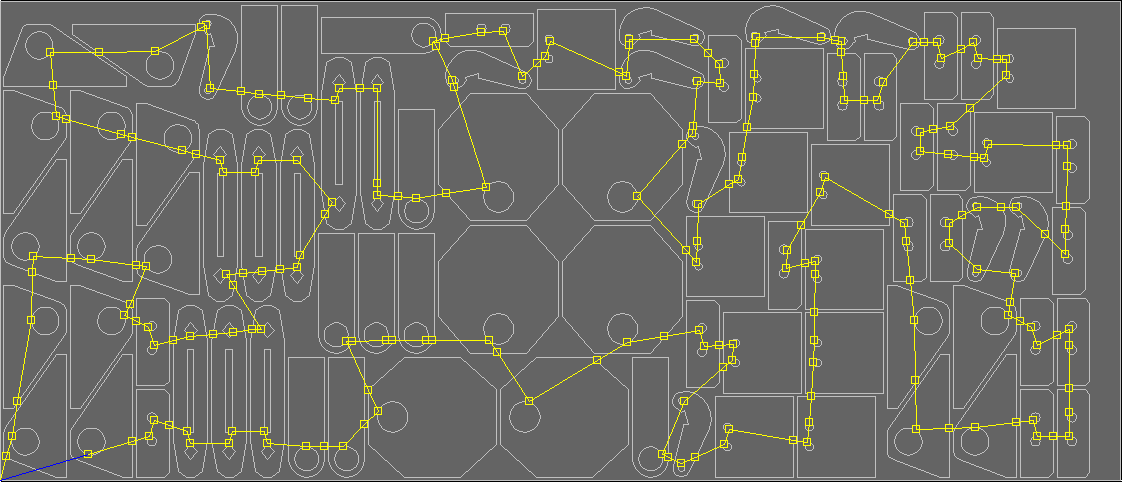
\includegraphics[angle=90,height=0.8\textheight]{dip_3.png}
  \end{center}
  \caption{Пример маршрута резки для большого количества контуров}
  \label{ccp-large}
\end{figure}

Для оценки качества решений,
получаемых описанным
эвристическим алгоритмом,
использовались несколько раскройных планов,
содержащих реальные детали.
В качестве базы сравнения
использовался алгоритм
(см. \cite{bi15}),
решающий задачу GTSP
(Generalized Traveling Salesman Problem,
Обобщённая задача коммивояжёра)
и дающий точное решение для количества контуров
$N \leqslant 33$.

На рис. \ref{gtsp-path}
показано точное решение задачи GTSP.
Хорошо видны возможные положения точек врезки,
которые получены путём дискретизации контура,
то есть сведения задачи непрерывной оптимизации
к задаче дискретной оптимизации.

\begin{figure}
  \begin{center}
    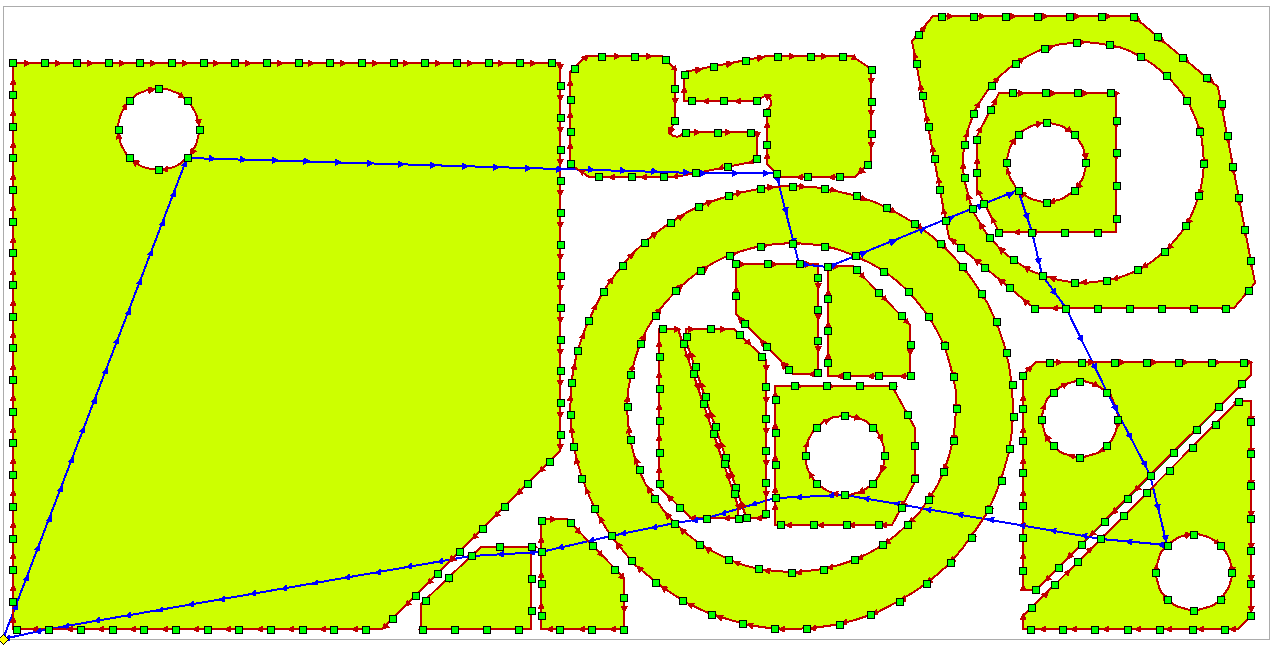
\includegraphics[width=0.95\textwidth]{464-gtsp.png}
  \end{center}
  \caption{Точное решение задачи GTSP для задания № 464}
  \label{gtsp-path}
\end{figure}

На рис. \ref{ccp-path}
показано решение задачи непрерывной резки,
полученное вышеописанным алгоритмом
для того же раскройного плана.

\begin{figure}
  \begin{center}
    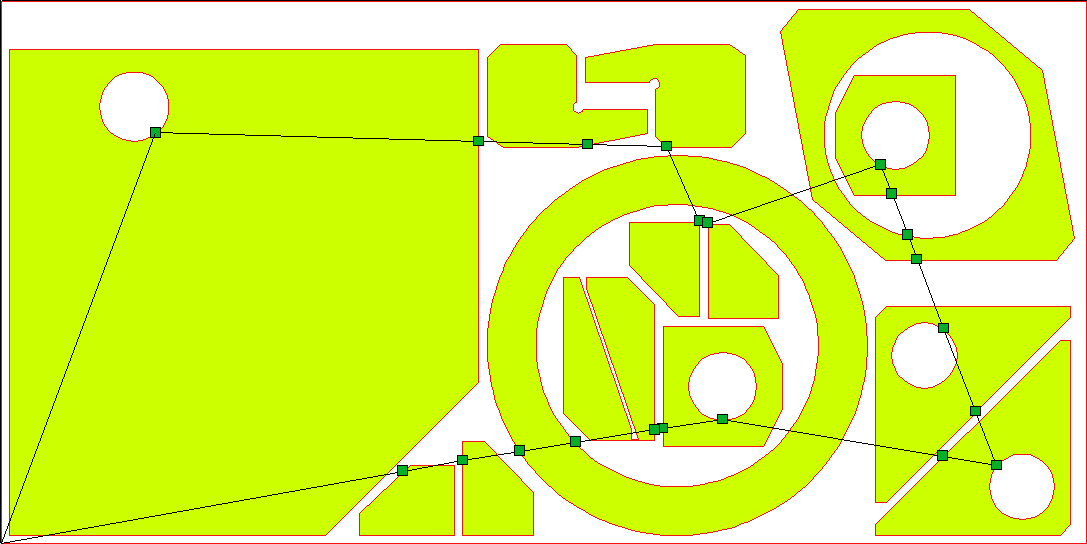
\includegraphics[width=0.95\textwidth]{464-ccp.png}
  \end{center}
  \caption{Решение задачи непрерывной резки для задания № 464}
  \label{ccp-path}
\end{figure}

Видно,
что оба алгоритма дают практически идентичные
маршруты резки.
Основное отличие вызвано необходимостью дискретизации
контуров в ходе сведения задачи
непрерывной резки к GTSP.
Характерной особенностью
решения задачи непрерывной резки
является то,
что оно
содержит много прямолинейных сегментов,
разделяемых точками врезки,
но фактически лежащих на одной прямой.
Аналогичные сегменты решения задачи GTSP
имеют небольшие изломы,
поскольку возможные координаты точек резки
фиксированы заранее и не могут попасть на одну прямую.
Поэтому общая длина холостого хода
в общем случае получается чуть больше,
чем для <<честного>> решения задачи непрерывной резки.
Подробнее это отображено в таблице
\ref{ccp-vs-gtsp}
для нескольких из использованных
раскройных планов.

\begin{table}[]
  \centering
  \begin{tabu} to 0.9\linewidth {X[2]|*{3}{X[r]}}
      Задание & № 229 & № 464 & № 3211 \\
      \hline
      Кол-во деталей & 11 & 14 & 17\\
      Кол-во контуров & 12 & 21 & 22 \\
      Общий периметер, м & 24.609 & 21.717 & 25.051 \\
      Кол-во точек GTSP & 491 & 429 & 493 \\
      $\mathcal L_{GTSP}$, м & 7.729 & 4.743 & 4.557 \\
      $\mathcal L_{CCP}$, м & 7.727 & 4.706 & 4.536 \\
      \hline
  \end{tabu}
  \caption{Сравнение качества решений задач CCP и GTSP}
  \label{ccp-vs-gtsp}
\end{table}

\begin{remark}
  Интересно,
  что
  \thref{cond2}
  соблюдено для всех контуров
  на рис. \ref{ccp-path},
  то есть изображённое там решение
  действительно представляет собой
  глобальнй минимум
  (длины холостого хода).
  В то же время,
  более простое
  \thref{cond2v}
  соблюдено для
  \textit{почти}
  всех контуров,
  кроме одного
  (невыпуклой детали сверху по центру).
  Это довольно редкая
  с практической точки зрения ситуация,
  тем не менее,
  она показывает,
  что две формулировки
  достаточного условия
  глобальности минимума
  не эквивалентны.
\end{remark}

На рис. \ref{ccp-large}
приведён
результат работы алгоритма
для раскройной карты с большим количеством
деталей
($n=82$)
и контуров
($N=219$).

\section{Заключение}

В данной работе был разработан
новый эвристический алгоритм решения
задачи непрерывной резки,
представлен способ
сведения данного класса задач
при наличии ограничения предшествования
к аналогичным задачам,
не имеющим такого ограничения,
разработана эвристика
поиска точек врезки в плоские контуры,
не использующая дискретизацию
и тем самым позволяющая уменьшить
полную длину холостого хода
режущего инструмента.
Для проведения комбинаторной оптимизации
в ходе алгоритма используется
хорошо описанный в литературе
подход переменных окрестностей
в пространстве перестановок.

Изучены маетматические свойства разработанной эвристики,
доказано,
что получаемый ею результат
доставляет локальный минимум
задачи непрерывной оптимизации
и представлены
\textit{достаточные}
и легко проверяемые
условия того,
что локальный минимум
является и глобальным.

Было разработано программное обеспечение на языке Си,
исполняющее данный алгоритм,
принимающее входные данные в стандартном
для современных CAD-систем формате.

Проведено исследование алгоритма
на раскройных планах,
применяемых в современном производстве,
в том числе в сравнении с уже
известными алгоритмами.
Продемонстрирована практическая применимость алгоритма,
быстродействие и хорошее качество
получаемых маршрутов режущего инструмента.

В качестве направлений дальнейших исследований
представляются следующие возможности:

\begin{itemize}
  \item
  Учёт того,
  что точка врезки размещается не на самом
  вырезаемом контуре,
  а на некоторой дистанции
  \textit{вне} его
  \item
  Учёт других технологических ограничений,
  порождаемых современным режущим оборудованием
  термической резки с ЧПУ,
  см. \cite{Sozopol}
  \item
  Разработка схемы использования разработанной эвристики
  совместно с другими алгоритмами комбинаторной оптимизации
  и оценка производительности и качества получаемых
  алгоритмов
\end{itemize}

\printbibliography[heading=bibintoc]
\nocite{*}

\end{document}
